\chapter{First-order self-energy and single-particle expectation values}
\label{first-order}

\section{Self-energy}
\label{first-order-self-energy}
The first-order diagram is
represented graphically as 
\begin{center}
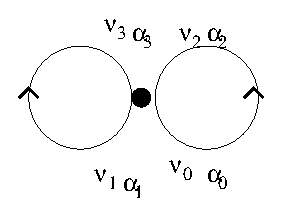
\epsfig{file=flex/phi_first.eps} 
\end{center}
and mathematically as
\begin{equation}
\Phi^{(1)} = \frac{T}{4} \sum_{\mathbf{r}_1} \int_0^{\beta}d\tau_1
\sum_{\nu_0\alpha_0\nu_1 \alpha_1\nu_2\alpha_2 \nu_3 \alpha_3} 
\Gamma^{(0)}_{\nu_0\alpha_0\nu_1\alpha_1; \nu_2\alpha_2 \nu_3\alpha_3}
G_{\nu_3\alpha_3\nu_1\alpha_1}(\tau_1,\mathbf{r}_1;\tau_1,\mathbf{r}_1)
\,G_{\nu_2\alpha_2\nu_0\alpha_0}(\tau_1,\mathbf{r}_1;\tau_1,\mathbf{r}_1) 
\end{equation}

The first order self-energy is obtained with
\begin{equation}
\Sigma^{(1)}_{\nu\alpha \nu^{\prime}\alpha^{\prime}}(x,x^{\prime})  =
T \frac{\delta\; \Phi^{(1)}}
{\delta\; G_{\nu^{\prime}\alpha^{\prime}\nu \alpha}(x^{\prime},x)} 
\end{equation}
which in this case yields
\begin{equation}
\begin{split}
\Sigma^{(1)}_{\nu\alpha \nu^{\prime}\alpha^{\prime}}(x,x^{\prime})
= & \frac{T^2}{2} \sum_{\nu_0\alpha_0 \nu_2\alpha_2;\nu_1 \alpha_1 \nu_3\alpha_3}
\int_{0}^{\beta}d\tau_1 \sum_{\mathbf{r}_1}
\Gamma^{(0)}_{\nu_0\alpha_0 \nu_1\alpha_1; \nu_2\alpha_2 \nu_3 \alpha_3}
G_{\nu_2\alpha_2\nu_0 \alpha_0}(\tau_1,\mathbf{r}_1;\tau_1,\mathbf{r}_1)
\delta_{\nu^{\prime}\alpha^{\prime},\nu_3\alpha_3}\,\delta_{\nu\alpha,\nu_1\alpha_1}
\delta_{\mathbf{r},\mathbf{r}_1} \delta_{\mathbf{r}^{\prime},\mathbf{r}_1} 
\\
& \times\,
\frac{\delta(\tau - \tau_1)}{T}\,\frac{\delta(\tau^{\prime} - \tau_1)}{T}
\end{split}
\end{equation}
which becomes
\begin{equation}
\Sigma^{(1)}_{\nu\alpha \nu^{\prime}\alpha^{\prime}}(x,x^{\prime}) =
\frac{1}{2}\sum_{\nu_0\alpha_0 \nu_2\alpha_2}
\Gamma^{(0)}_{\nu_0\alpha_0\nu\alpha; \nu_2\alpha_2 \nu^{\prime}\alpha^{\prime}}
G_{\nu_2\alpha_2 \nu_0\alpha_0}(\tau,\mathbf{r};\tau,\mathbf{r})\,
\delta_{\mathbf{r},\mathbf{r}^{\prime}} \, \delta(\tau - \tau^{\prime})
\end{equation}
Graphically, this self energy is represented as\\
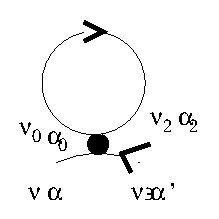
\epsfig{file=flex/sigma_first.eps}\\
The overall positive sign comes from having a (-1) from one
occurence of the interaction and another (-1) for having
a closed loop.

For a translationally invariant system we have (after changing
the internal subscript ``2'' to ``1'')
\begin{equation}
\Sigma^{(1)}_{\nu\alpha \nu^{\prime}\alpha^{\prime}}(\tau,\mathbf{r}) =
\frac{1}{2} \sum_{\nu_0\alpha_0 \nu_1\alpha_1}
\Gamma^{(0)}_{\nu_0\alpha_0\alpha;\nu_1 \alpha_1 \nu^{\prime}\alpha^{\prime}}
G_{\nu_1\alpha_1 \nu_0\alpha_0}(\tau=0,\mathbf{r}=\mathbf{0})\,
\delta_{\mathbf{r},\mathbf{0}} \, \delta(\tau)
\end{equation}
There is an ambiguity as to whether take $\tau \to 0^+$ or
$\tau \to 0^-$.  If $\alpha_1 \neq \alpha_0$ and/or $\nu_1 \neq \nu_0$, 
then this
ambiguity is irrelevant.  However, if $\alpha_1 = \alpha_0$
and $\nu_1 = \nu_0$,
then the $\tau \to 0^-$ limit should be used if $\alpha_0$
and $\alpha_1$ correspond to particle degrees of freedom (0,1)
and $\tau \to 0^+$ should be used for hole degrees of freedom
(2,3).

Since the self-energy is local in time and space, its Fourier
transform is independent of frequency and momentum.  We have
\begin{eqnarray}
\Sigma^{(1)}_{\nu\alpha \nu^{\prime}\alpha^{\prime}}(\epsilon_n,\mathbf{k}) \equiv
\Sigma^{(1)}_{\nu\alpha \nu^{\prime}\alpha^{\prime}} &  = &
\frac{1}{2} \sum_{\nu_0\alpha_0 \nu_1\alpha_1}
\Gamma^{(0)}_{\nu_0\alpha_0\nu\alpha; \nu_1\alpha_1 \nu^{\prime}\alpha^{\prime}}
G_{\nu_1\alpha_1 \nu_0\alpha_0}(\tau=0,\mathbf{r}=\mathbf{0}) \\
& = & \frac{1}{2} \sum_{\nu_0\alpha_0 \nu_1\alpha_1}
\Gamma^{(0)ph}_{\nu_0 \alpha_0 \nu_1 \alpha_1;
\nu^{\prime}\alpha^{\prime} \nu \alpha}
G_{\nu_1\alpha_1 \nu_0\alpha_0}(\tau=0,\mathbf{r}=\mathbf{0})
\end{eqnarray}

For concretness, consider the single band case to see how the above formula
is able to reproduce well know results.
Using the definition of $\Gamma^{(0)}$ from Chapter~\ref{chapter:bare_vertex},
we obtain the following explicit forms for the $\Sigma^{(1)}$
where the spatial part of the Green's function is assumed to
be evaluated at $\mathbf{r} = \mathbf{0}$:
\begin{eqnarray}
\Sigma^{(1)}_{00} & = &
\frac{1}{2}\sum_{\alpha_0\beta_0} \Gamma^{(0)}_{\alpha_0 0; \beta_0 0}
G_{\beta_0 \alpha_0}(\tau =0, \mathbf{r}=\mathbf{0}) \\
    & = & \frac{1}{2}\left(U G_{11}(\tau = 0^-) - 
        U G_{33}(\tau = 0^+) \right)\\
    & = & U\, G_{11}(\tau = 0^-) 
\end{eqnarray}
\begin{eqnarray}
\Sigma^{(1)}_{01} & = &
\frac{1}{2}\sum_{\alpha_0\beta_0} \Gamma^{(0)}_{\alpha_0 0; \beta_0 1}
G_{\beta_0 \alpha_0}(\tau =0, \mathbf{r}=\mathbf{0}) \\
    & = & \frac{1}{2}\left(-U G_{01}(\tau = 0) + 
U G_{32}(\tau = 0)\right) \\
    & = & -U\, G_{01}(\tau = 0)
\end{eqnarray}
\begin{eqnarray}
\Sigma^{(1)}_{02} & = &
\frac{1}{2}\sum_{\alpha_0\beta_0} \Gamma^{(0)}_{\alpha_0 0; \beta_0 2}
G_{\beta_0 \alpha_0}(\tau =0, \mathbf{r}=\mathbf{0}) \\
    & = & 0  \;\;\textrm{(no non-zero vertices)}
\end{eqnarray}
\begin{eqnarray}
\Sigma^{(1)}_{03} & = &
\frac{1}{2}\sum_{\alpha_0\beta_0} \Gamma^{(0)}_{\alpha_0 0; \beta_0 3}
G_{\beta_0 \alpha_0}(\tau =0, \mathbf{r}=\mathbf{0}) \\
    & = & \frac{1}{2}\left(-U G_{12}(\tau = 0) + U G_{03}(\tau = 0)\right) \\
    & = & U\, G_{03}(\tau = 0) 
\end{eqnarray}
\begin{eqnarray}
\Sigma^{(1)}_{10} & = &
\frac{1}{2}\sum_{\alpha_0\beta_0} \Gamma^{(0)}_{\alpha_0 1; \beta_0 0}
G_{\beta_0 \alpha_0}(\tau =0, \mathbf{r}=\mathbf{0}) \\
    & = & \frac{1}{2}\left(-U G_{10}(\tau = 0) + 
U G_{23}(\tau = 0)\right) \\
    & = & -U\, G_{10}(\tau = 0)
\end{eqnarray}
\begin{eqnarray}
\Sigma^{(1)}_{11} & = &
\frac{1}{2}\sum_{\alpha_0\beta_0} \Gamma^{(0)}_{\alpha_0 1; \beta_0 1}
G_{\beta_0 \alpha_0}(\tau =0, \mathbf{r}=\mathbf{0}) \\
    & = & \frac{1}{2}\left(U G_{00}(\tau = 0^-)  
- U G_{22}(\tau = 0^+)\right) \\
    & = & U\, G_{00}(\tau = 0^-)
\end{eqnarray}
\begin{eqnarray}
\Sigma^{(1)}_{12} & = &
\frac{1}{2}\sum_{\alpha_0\beta_0} \Gamma^{(0)}_{\alpha_0 1; \beta_0 2}
G_{\beta_0 \alpha_0}(\tau =0, \mathbf{r}=\mathbf{0}) \\
    & = & \frac{1}{2}\left(U G_{12}(\tau = 0) 
- U G_{03}(\tau = 0)\right) \\
    & = & -U\, G_{03}(\tau = 0)
\end{eqnarray}
\begin{eqnarray}
\Sigma^{(1)}_{22} & = &
\frac{1}{2}\sum_{\alpha_0\beta_0} \Gamma^{(0)}_{\alpha_0 2; \beta_0 2}
G_{\beta_0 \alpha_0}(\tau =0, \mathbf{r}=\mathbf{0}) \\
    & = & \frac{1}{2}\left(-U G_{11}(\tau = 0^-) + 
U G_{33}(\tau = 0^+)\right) \\
    & = & -U\, G_{11}(\tau = 0^-) = -\Sigma^{(1)}_{00} 
\end{eqnarray}
In matrix form $\Sigma^{(1)}$ is given by
\begin{equation}
\Sigma^{(1)} = 
U 
\begin{pmatrix}
G_{11} & -G_{01} & 0 & G_{03} \\
-G_{10} & G_{00} & -G_{03} & 0 \\
0  & -G_{30} & -G_{11} & G_{10} \\
G_{30} & 0 & G_{01} & -G_{00}
\end{pmatrix}
\end{equation}

\section{$\mathrm{Tr}\; \Sigma^{(1)} G$}

This trace is needed in the evaluation of the thermodynamic
potential.  For this trace we have
\begin{eqnarray}
\mathrm{Tr}\; \Sigma^{(1)} G & \equiv &
      T \sum_{\mathbf{k},\varepsilon_n}
 \textrm{Tr}\, \Sigma^{(1)}\, 
G(\varepsilon_n,\mathbf{k})
\\
& = & 
  N_{sites} 
\mathrm{Tr}\; \Sigma^{(1)} G(\tau=0,\mathbf{r}=\mathbf{0}) \\
 & = &   N_{sites} 
\mathrm{Tr}\; U
\begin{pmatrix}
G_{11} & -G_{01} & 0 & G_{03} \\
-G_{10} & G_{00} & -G_{03} & 0 \\
0  & -G_{30} & -G_{11} & G_{10} \\
G_{30} & 0 & G_{01} & -G_{00}
\end{pmatrix}
\begin{pmatrix}
G_{00} & G_{01} & G_{02} & G_{03} \\
G_{10} & G_{11} & G_{12} & G_{13} \\
G_{20}  & G_{21} & G_{22} & G_{23} \\
G_{30} & G_{31} & G_{32} & G_{33}
\end{pmatrix}
\\
& = &
 N_{sites} 
\mathrm{Tr}\; U
\begin{pmatrix}
G_{11} & -G_{01} & 0 & G_{03} \\
-G_{10} & G_{00} & -G_{03} & 0 \\
0  & -G_{30} & -G_{11} & G_{10} \\
G_{30} & 0 & G_{01} & -G_{00}
\end{pmatrix}
\begin{pmatrix}
G_{00} & G_{01} & G_{02} & G_{03} \\
G_{10} & G_{11} & -G_{03} & G_{13} \\
G_{20}  & -G_{30} & -G_{00} & G_{23} \\
G_{30} & G_{31} & G_{32} & -G_{11}
\end{pmatrix}
\\
& = & 4 N_{sites} U (G_{11}G_{00} - G_{01}G_{10} + G_{03}G_{30}) 
\end{eqnarray}
In the above we have used the symmetries of the Green's function
described in Chapter~\ref{chapter:g0}.

The last term in the above gives the BCS-like contribution to
the condensation energy for an $s$-wave superconductor.  The 
first term is the normal Hartree energy, $<n_{\uparrow}><n_{\downarrow}>$.
The nature of the middle term is more clear when we note that
\begin{eqnarray}
G_{00} & = & \frac{1}{2}( n + m_z) \\
G_{11} & = & \frac{1}{2}( n - m_z) \\
G_{01} & = & \frac{1}{2}( m_x + i m_y) \\
G_{10} & = & \frac{1}{2}( m_x - i m_y)
\end{eqnarray}
Upon substitution we find that
\begin{equation}
\mathrm{Tr}\; \Sigma^{(1)} G = 4 N_{sites} U 
\left( \frac{1}{4} n^2 - \frac{1}{4}(m_x^2 + m_y^2 + m_z^2)
+ G_{03}G_{30} \right)
\end{equation}
Thus, the $G_{01}G_{10}$ term is needed to account for
polarization in the $x$ or $y$ directions.

\section{Evaluation of average single-particle energies}

The average value of the kinetic energy is easiest
to evaluate in $\mathbf{k}$-space.  We have
\begin{eqnarray}
\frac{<KE>}{N_L} & = & \frac{1}{N_L}
\sum_{\mathbf{k}\nu\nu^{\prime}\sigma} \epsilon_{\nu\nu^{\prime}}(\mathbf{k}) 
<c^{\dagger}_{\mathbf{k}\nu\sigma} c_{\mathbf{k}\nu^{\prime}\sigma}>
\\
& = & \frac{1}{N_L} \sum_{\mathbf{k}\nu\nu^{\prime}\sigma} 
\epsilon_{\nu\nu^{\prime}}(\mathbf{k}) 
G_{\nu^{\prime}\sigma \nu\sigma}(\tau \to 0^-, \mathbf{k}) 
\end{eqnarray}

The magnetic field coupling energy is simplest to evaluate
in real-space.  There it is given by
\begin{eqnarray}
\frac{<E_{mag}>}{N_L} & = & - \frac{1}{N_L} 
\sum_{\mathbf{r}\nu\sigma\sigma^{\prime}} \mathbf{h}\cdot 
\vec{\sigma}_{\sigma\sigma^{\prime}}
 <c^{\dagger}_{\mathbf{r}\nu\sigma} c_{\mathbf{r}\nu\sigma^{\prime}}>
 \\
& = & - \sum_{\nu\sigma\sigma^{\prime}} 
\mathbf{h}\cdot\vec{\sigma}_{\sigma\sigma^{\prime}}\,
G_{\nu\sigma^{\prime}\nu\sigma}(\tau \to 0^-,\mathbf{r} = \mathbf{0}) 
\end{eqnarray}.

\section{Updating $\phi(\mathbf{r})$}

Recall that
\begin{equation}
H_{p}  = -h_p\frac{\sqrt{N_l}}{2} 
\left( \sum_{\mathbf{r}\mathbf{r}^{\prime}
\nu\nu^{\prime}\sigma\sigma^{\prime}}  
\Psi_{\nu\sigma\nu^{\prime}\sigma^{\prime}}(\mathbf{r},\mathbf{r}^{\prime})
 c_{\mathbf{r}\nu\sigma}c_{\mathbf{r}^{\prime}\nu^{\prime}\sigma^{\prime}} + 
\Psi_{\nu^{\prime}\sigma^{\prime}\nu\sigma}^*(\mathbf{r}^{\prime},\mathbf{r})
c^{\dagger}_{\mathbf{r}\nu\sigma}
 c^{\dagger}_{\mathbf{r}^{\prime}\nu^{\prime}\sigma^{\prime}}\right)
\end{equation}
so that
\begin{equation}
E_p \equiv <H_p> 
= -h_p\frac{\sqrt{N_l}}{2} 
\left( \sum_{\mathbf{r}\mathbf{r}^{\prime}\nu\nu^{\prime}\sigma\sigma^{\prime}}  
\Psi_{\nu\sigma\nu^{\prime}\sigma^{\prime}}(\mathbf{r},\mathbf{r}^{\prime})
<c_{\mathbf{r}\nu\sigma}c_{\mathbf{r}^{\prime}\nu^{\prime}\sigma^{\prime}}> + 
\Psi_{\nu^{\prime}\sigma^{\prime}\nu\sigma}^*(\mathbf{r}^{\prime},\mathbf{r})
 <c^{\dagger}_{\mathbf{r}\nu\sigma}
 c^{\dagger}_{\mathbf{r}^{\prime}\nu^{\prime}\sigma^{\prime}}>\right)
\end{equation}
The expectation values represents the
equal-time, spatially-dependent
induced pairing magnitude.
We define the \textit{induced} pairing state, $\Psi^{\prime}$
and \textit{induced} pairing amplitude, $m_p $, by
\begin{equation}
<c_{\mathbf{r}\nu\sigma}c_{\mathbf{r}^{\prime}\nu^{\prime}\sigma^{\prime}}>  =  m_p 
\left(\Psi^{\prime}_{\nu^{\prime}\sigma^{\prime}\mu\sigma}(\mathbf{r}^{\prime},
\mathbf{r})\right)^* \sqrt{N_l}
\end{equation}
which implies that
\begin{equation}
<c^{\dagger}_{\mathbf{r}\nu\sigma} 
c^{\dagger}_{\mathbf{r}^{\prime}\nu^{\prime}\sigma^{\prime}}>  = 
m_p \Psi^{\prime}_{\nu\sigma\nu^{\prime}\sigma^{\prime}}(\mathbf{r},\mathbf{r}^{\prime})
\sqrt{N_l}.
\end{equation}
\begin{eqnarray}
E_p & =  & - h_p m_p \frac{N_l}{2} 
\sum_{\mathbf{r}\mathbf{r}^{\prime}\nu\nu^{\prime}\sigma\sigma^{\prime}} 
\Psi_{\nu\sigma\nu^{\prime}\sigma^{\prime}}(\mathbf{r},\mathbf{r}^{\prime}) 
\left(\Psi^{\prime}_{\nu^{\prime}\sigma^{\prime}\nu\sigma}
(\mathbf{r}^{\prime},\mathbf{r})\right)^* +
\left(\Psi_{\nu^{\prime}\sigma^{\prime}\nu\sigma}(\mathbf{r}^{\prime},
\mathbf{r})\right)^* 
\Psi^{\prime}_{\nu\sigma\nu^{\prime}\sigma^{\prime}}(\mathbf{r},\mathbf{r}^{\prime})
\\
& = &
- h_p m_p N_l \;\textrm{Re }
\left(\sum_{\mathbf{r}\mathbf{r}^{\prime}\nu\nu^{\prime}\sigma\sigma^{\prime}} 
\Psi_{\nu\sigma\nu\sigma^{\prime}}(\mathbf{r},\mathbf{r}^{\prime}) 
\left(\Psi^{\prime}_{\nu^{\prime}\sigma^{\prime}\nu\sigma}
(\mathbf{r}^{\prime},\mathbf{r})\right)^* \right)  
\end{eqnarray} 
For a translationally invariant system this reduces to
\begin{equation}
\frac{<E_p>}{N_l}  =  - 
h_p m_p\;\textrm{Re } \sum_{\mathbf{r}\nu\nu^{\prime}\sigma\sigma^{\prime}}
    \phi_{\nu\sigma\nu^{\prime}\sigma^{\prime}}(\mathbf{r}) 
\left(\phi^{\prime}_{\nu^{\prime}\sigma^{\prime}\nu\sigma}(-\mathbf{r})\right)^* 
\end{equation}

To find the strongest pairing channel, we want the applied
pair field to couple directly to the induced pairing wave function,
\textit{i.e.} $\phi = \phi^{\prime}$.  Thus, on each iteration
we determine $\phi^{\prime}$ from
\begin{equation}
<c^{\dagger}_{\mathbf{r}^{\prime}\nu^{\prime}\sigma^{\prime}} 
c^{\dagger}_{\mathbf{r}\nu\sigma}> = 
m_p \Psi^{\prime}_{\nu\sigma\nu^{\prime}\sigma^{\prime}}(\mathbf{r},\mathbf{r}^{\prime}) \sqrt{N_l}
\end{equation}
so that in the translationally invariant case (and assuming
$n_p = 0$)
\begin{equation} 
<c^{\dagger}_{\mathbf{r}^{\prime}\nu^{\prime}\sigma^{\prime}} 
c^{\dagger}_{\mathbf{r}\nu\sigma}>  =  m_p 
\,\phi_{\nu\sigma\nu^{\prime}\sigma^{\prime}}^{\prime}(\mathbf{r} -
\mathbf{r}^{\prime}) 
\end{equation}
The left hand side is obtained from the equal time Green's
function.  Namely
\begin{eqnarray} 
<c^{\dagger}_{\mathbf{r}^{\prime}\nu^{\prime}\sigma^{\prime}} 
c^{\dagger}_{\mathbf{r}\nu\sigma}> & \equiv &
<\psi^{\dagger}_{\mathbf{r}^{\prime}\nu^{\prime}\sigma^{\prime}}
\psi_{\mathbf{r}\nu\overline{\sigma}}> \\
& = & 
G_{\nu\overline{\sigma}\nu^{\prime}\sigma^{\prime}}(\mathbf{r}-\mathbf{r}^{\prime},
\tau \to 0-).
\end{eqnarray}

Thus, $\phi_{\nu\sigma\nu^{\prime}\sigma^{\prime}}(\mathbf{r})$ 
is obtained by normalizing  
$G_{\nu\overline{\sigma}\nu^{\prime}\sigma^{\prime}}(\tau \to 0^-, \mathbf{r})$.
The normalization constant is the pairing strength, $m_p$.
Finally, to iterate our pairing field 
to the strongest pairing channel, we set
$\phi = \phi^{\prime}$ on each iteration
as new results for $G(\tau \to 0^-, \mathbf{r})$
are computed.  
